%\documentclass[9pt]{scrartcl}
\documentclass[a4paper]{article}
\usepackage[]{amsmath}
\usepackage{tikz}
\usetikzlibrary{positioning}
%\usepackage{helvet}
\usepackage{listings}
\usepackage{geometry}
%\geometry{textheight=\paperheight, noheadfoot, nomarginpar}
\usetikzlibrary{positioning,shapes,shadows}
\renewcommand{\familydefault}{\sfdefault}

\tikzstyle{abstract}=[rectangle, draw=black, fill=gray!20, text centered,  text=black, text width=12.5mm]
\tikzstyle{spacestyle}=[rectangle, draw=black, fill=gray!20, text centered,  text=black, text width=50mm]

\lstset{
        language=python,
        basicstyle=\fontencoding{T1}\ttfamily,
        commentstyle=\color{gray},
        keywordstyle=\color{OliveGreen},
        frame=single,
        backgroundcolor=\color{lightlightgray},
        tabsize=2,
        %deletestring=[d]",
        %escapechar=\%,
        numbers=left,
        showstringspaces=false,
}
\usepackage[explicit]{titlesec} 
\titleformat{\section}{\normalfont\Large\bfseries}{}{0em}{#1}
\titleformat{\subsection}{\normalfont\bfseries}{}{0em}{--#1}

\newcommand{\arrow}[4]{%
\draw[-latex, thick,#4] ([yshift=-0.6 *\they cm-0.5  cm] #1.south) -- ([yshift=-0.6*\they cm-0.9 cm] #2.south) node[midway,above right] {#3};%
} 
\newcommand{\arrowred}[3]{%
\draw[-latex, thick, red] ([yshift=-0.6 *\they cm-0.5  cm] #1.south) -- ([yshift=-0.6*\they cm-0.9 cm] #2.south) node[midway,above right] {#3};%
} 
\newcommand{\arrowfar}[4]{%
\draw[-latex, thick, #4] ([yshift=-0.6 *\they cm-0.5  cm] #1.south) -- ([yshift=-0.6*\they cm-1.5 cm] #2.south) node[midway,above right] {#3};%
} 
\newcommand{\arrowredfar}[3]{%
\draw[-latex, thick,red] ([yshift=-0.6 *\they cm-0.5  cm] #1.south) -- ([yshift=-0.6*\they cm-1.5 cm] #2.south) node[midway,above right] {#3};%
} 

\newcommand{\mykey}[2]{%
\begin{tikzpicture} \node (Item) [abstract, minimum size=12.5mm, align=center]
{\vrule height 12pt depth 8pt width 0pt\textbf{#1} \\\vrule height 6pt depth 8pt width 0pt\parbox{1.25cm}{\centering{\fontsize{6pt}{8pt}\selectfont{#2}}}};%
\end{tikzpicture}}


\begin{document}
\begin{center}
\Large{Diagram}
\end{center}
\noindent%


\section {System diagram}

Write operation structure:\\\\
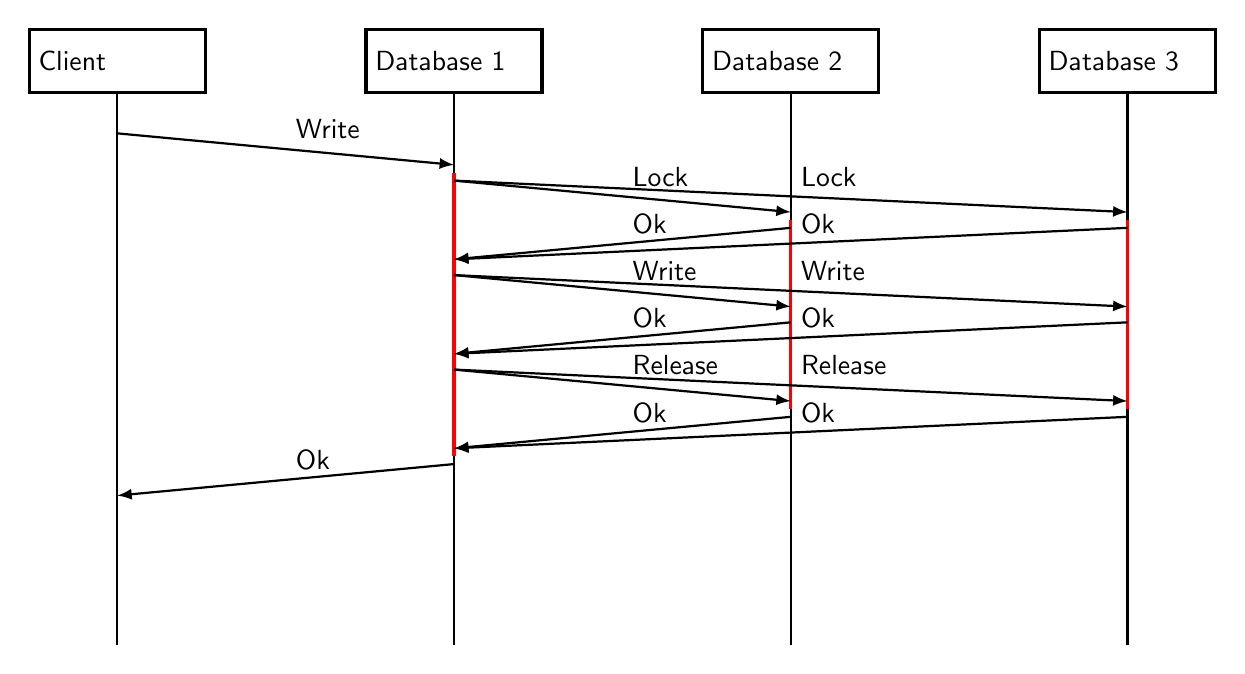
\begin{tikzpicture}

% Client
\node [draw,
	minimum width=2cm,
	minimum height=0.8cm,
	text width=2cm,
	very thick,
]  (client) {
Client
};

% Database 1
\node [draw,
	minimum width=2cm,
	minimum height=0.8cm,
	text width=2cm,
	very thick,
	right = 2cm of client
]  (db1) {
Database 1
};
% Database 2
\node [draw,
	minimum width=2cm,
	minimum height=0.8cm,
	text width=2cm,
	very thick,
	right = 2cm of db1
]  (db2) {
Database 2
};

% Database 3
\node [draw,
	minimum width=2cm,
	minimum height=0.8cm,
	text width=2cm,
	very thick,
	right = 2cm of db2
]  (db3) {
Database 3
};

% Arrows with text label

\draw[thick] (client.south) -- ([yshift=-7cm] client.south);
\draw[thick] (db1.south) -- ([yshift=-7cm] db1.south);
\draw[thick] (db2.south) -- ([yshift=-7cm] db2.south);
\draw[thick] (db3.south) -- ([yshift=-7cm] db3.south);
\draw[very thick,red] ([yshift=-1.6cm]db3.south) -- ([yshift=-4cm] db3.south);
\draw[very thick,red] ([yshift=-1.6cm]db2.south) -- ([yshift=-4cm] db2.south);
\draw[very thick,red] ([yshift=-1cm]db1.south) -- ([yshift=-4.6cm] db1.south);

\newcounter{y}
\arrow{client}{db1}{Write}{black}
\stepcounter{y};

\arrow{db1}{db2}{Lock}{black}
\arrow{db1}{db3}{Lock}{black}
\stepcounter{y};
\arrow{db2}{db1}{Ok}{black}
\arrow{db3}{db1}{Ok}{black}
\stepcounter{y};

\arrow{db1}{db2}{Write}{black}
\arrow{db1}{db3}{Write}{black}
\stepcounter{y};
\arrow{db2}{db1}{Ok}{black}
\arrow{db3}{db1}{Ok}{black}
\stepcounter{y};

\arrow{db1}{db2}{Release}{black}
\arrow{db1}{db3}{Release}{black}
\stepcounter{y};
\arrow{db2}{db1}{Ok}{black}
\arrow{db3}{db1}{Ok}{black}
\stepcounter{y};

\arrow{db1}{client}{Ok}{}

\end{tikzpicture}

\pagebreak
\noindent
Write operation structure with simultaneous writes, green is randomly given higher priority:\\\\
\begin{tikzpicture}

% Client
\node [draw,
	minimum width=2cm,
	minimum height=0.8cm,
	text width=2cm,
	very thick,
]  (client) {
Client 1
};

% Database 1
\node [draw,
	minimum width=2cm,
	minimum height=0.8cm,
	text width=2cm,
	very thick,
	right = 1cm of client
]  (db1) {
Database 1
};
% Database 2
\node [draw,
	minimum width=2cm,
	minimum height=0.8cm,
	text width=2cm,
	very thick,
	right = 1cm of db1
]  (db2) {
Database 2
};

% Database 3
\node [draw,
	minimum width=2cm,
	minimum height=0.8cm,
	text width=2cm,
	very thick,
	right = 1cm of db2
]  (db3) {
Database 3
};
% Client2
\node [draw,
	minimum width=2cm,
	minimum height=0.8cm,
	text width=2cm,
	very thick,
	right = 1cm of db3
]  (client2) {
Client 2
};

% Arrows with text label

\draw[thick] (client.south) -- ([yshift=-10cm] client.south);
\draw[thick] (db1.south) -- ([yshift=-10cm] db1.south);
\draw[thick] (db2.south) -- ([yshift=-10cm] db2.south);
\draw[thick] (db3.south) -- ([yshift=-10cm] db3.south);
\draw[thick] (client2.south) -- ([yshift=-10cm] client2.south);
\draw[very thick,blue] ([yshift=-1cm]db3.south) -- ([yshift=-3cm] db3.south);
\draw[very thick,green] ([yshift=-3.4cm]db3.south) -- ([yshift=-4.6cm] db3.south);
\draw[very thick,green] ([yshift=-1.6cm]db2.south) -- ([yshift=-4.6cm] db2.south);
\draw[very thick,green] ([yshift=-1cm]db1.south) -- ([yshift=-4cm] db1.south);
\draw[very thick,blue] ([yshift=-5cm]db3.south) -- ([yshift=-7.6cm] db3.south);
\draw[very thick,blue] ([yshift=-5.8cm]db2.south) -- ([yshift=-8.2cm] db2.south);
\draw[very thick,blue] ([yshift=-5.8cm]db1.south) -- ([yshift=-8.2cm] db1.south);

\setcounter{y}0
\arrow{client}{db1}{Write}{green}
\arrow{client2}{db3}{Write}{blue}
\stepcounter{y};

\arrow{db1}{db2}{Lock}{green}
\arrowfar{db1}{db3}{Lock}{green}
\arrowfar{db3}{db2}{Lock}{blue}
\arrow{db3}{db1}{Lock}{blue}
\stepcounter{y};
\arrow{db2}{db1}{Ok}{green}
\arrowredfar{db1}{db3}{}
\stepcounter{y};
\arrowred{db2}{db3}{}
\stepcounter{y};

\arrow{db3}{db2}{Release}{blue}
\arrow{db3}{db1}{Release}{blue}
\stepcounter{y};
\arrow{db2}{db3}{Ok}{blue}
\arrow{db1}{db3}{Ok}{blue}
\arrow{db3}{db1}{Ok}{green}
\stepcounter{y};
\arrow{db1}{db2}{Release}{green}
\arrow{db1}{db3}{Release}{green}
\stepcounter{y};
\arrow{db2}{db1}{Ok}{green}
\arrow{db3}{db1}{Ok}{green}
\stepcounter{y};

\arrow{db1}{client}{Ok}{green}
\arrow{db3}{db2}{Lock}{blue}
\arrow{db3}{db1}{Lock}{blue}
\stepcounter{y};
\arrow{db2}{db3}{Ok}{blue}
\arrow{db1}{db3}{Ok}{blue}
\stepcounter{y};

\arrow{db3}{db2}{Write}{blue}
\arrow{db3}{db1}{Write}{blue}
\stepcounter{y};
\arrow{db2}{db3}{Ok}{blue}
\arrow{db1}{db3}{Ok}{blue}
\stepcounter{y};

\arrow{db3}{db2}{Release}{blue}
\arrow{db3}{db1}{Release}{blue}
\stepcounter{y};
\arrow{db2}{db3}{Ok}{blue}
\arrow{db1}{db3}{Ok}{blue}
\stepcounter{y};
\arrow{db3}{client2}{Ok}{blue}



\end{tikzpicture}


\end{document}